\section{Problem komiwojażera}

Do badań zostały wykorzystane trzy instancje US50, bay29 i brg180. Wpływ zmiany parametrów potwierdził słuszność domyślnych ustawień pakietu GA. Dodatkowo w tym sprawozdaniu potwierdzają się również wnioski wysnute w sprawozdaniu nr 1.


\subsection{Kod źródłowy}

\begin{lstlisting}[linewidth=15.4cm]
data("USCA50")
D <- as.matrix(USCA50)
d <- USCA50


tourLength <- function(tour, distMatrix) {
   tour <- c(tour, tour[1])
   route <- embed(tour, 2)[, 2:1]
   sum(distMatrix[route])
}

tpsFitness <- function(tour, ...) 1/tourLength(tour, ...)

meanGA <- function(population,iteration,crosing,mutant,inst,elit, D)
{
   xMax <- matrix ( 0 ,iteration,15)   
   xMean <- matrix ( 0 ,iteration,15)  

   for ( i in 1:15)
   {  
	GA <- ga(type = "permutation",
	fitness = tpsFitness ,
	min = 1,distMatrix = D, max =attr(inst, "Size"), 
	pcrossover = crosing, pmutation = mutant,
	popSize = population, maxiter = iteration,elitism = elit )
	xMax[,i] <- 1/GA@summary[,1]
	xMean[,i] <- 1/GA@summary[,2]
	print(GA@solution)
   }

   return(list(max=xMax,min=xMean))

}
gaResult <- meanGA(100,50,0.5,0.1,d,5,D)
meanRowsMax <- rowMeans(gaResult$max )
meanRowsMean <- rowMeans(gaResult$min)
\end{lstlisting}


\subsection{Krzyżowanie}


\begin{figure}[H]
\centering

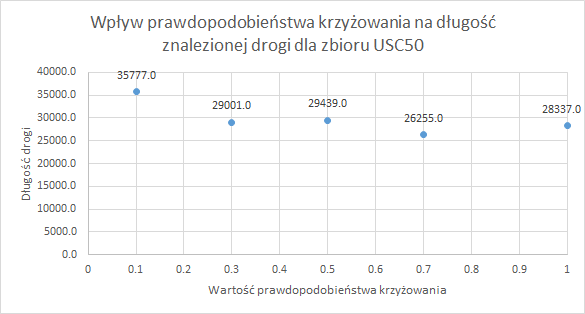
\includegraphics[scale=0.9]{IO_obrazy/excel_usca_kros}
\end{figure}


\begin{figure}[H]
\centering

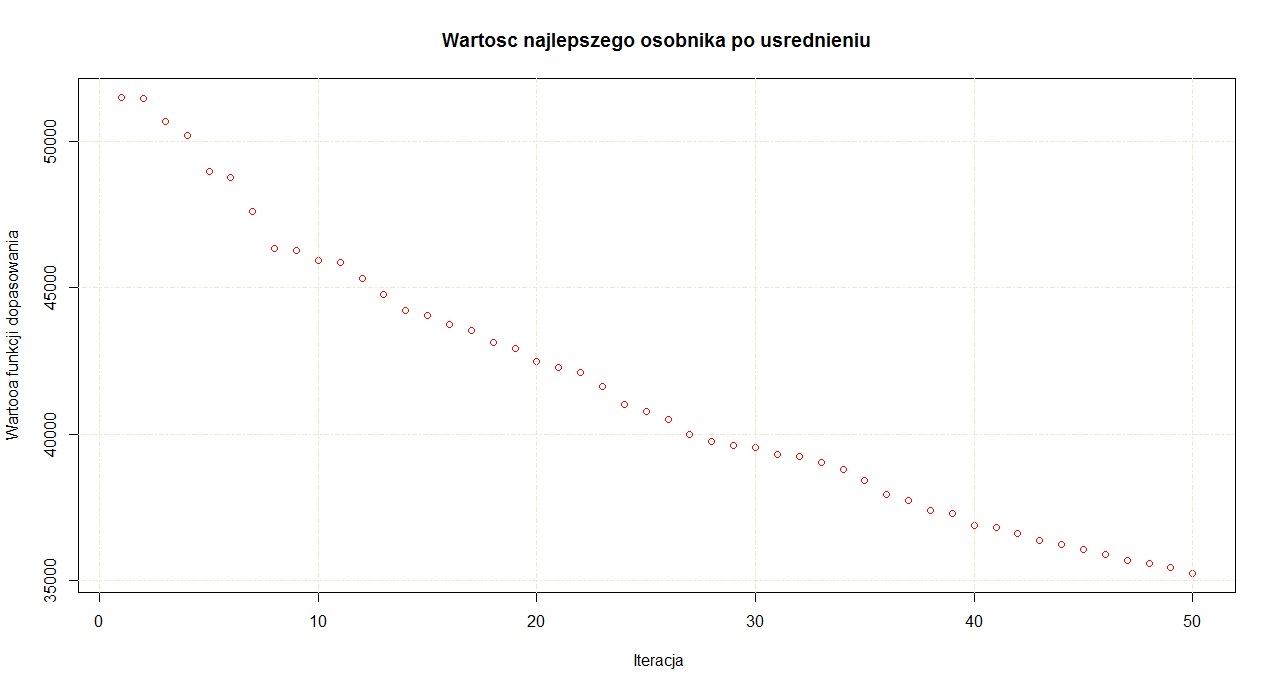
\includegraphics[scale=0.3]{IO_obrazy/US50_krz_01}
\caption{Wykres wartości najlepszego osobnika dla prawdopodobieństwa krzyżowania równego 0.1}
\end{figure}

\begin{figure}[H]
\centering

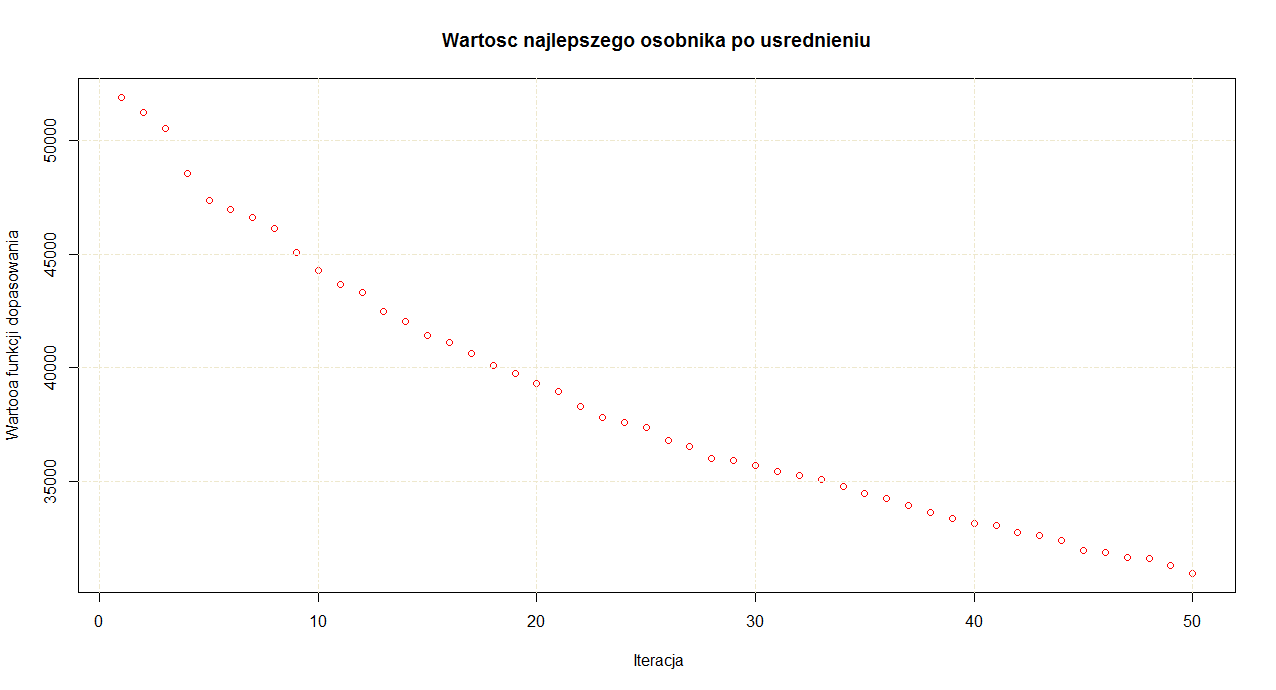
\includegraphics[scale=0.3]{IO_obrazy/US50_krz_03}
\caption{Wykres wartości najlepszego osobnika dla prawdopodobieństwa krzyżowania równego 0.3}
\end{figure}

\begin{figure}[H]
\centering

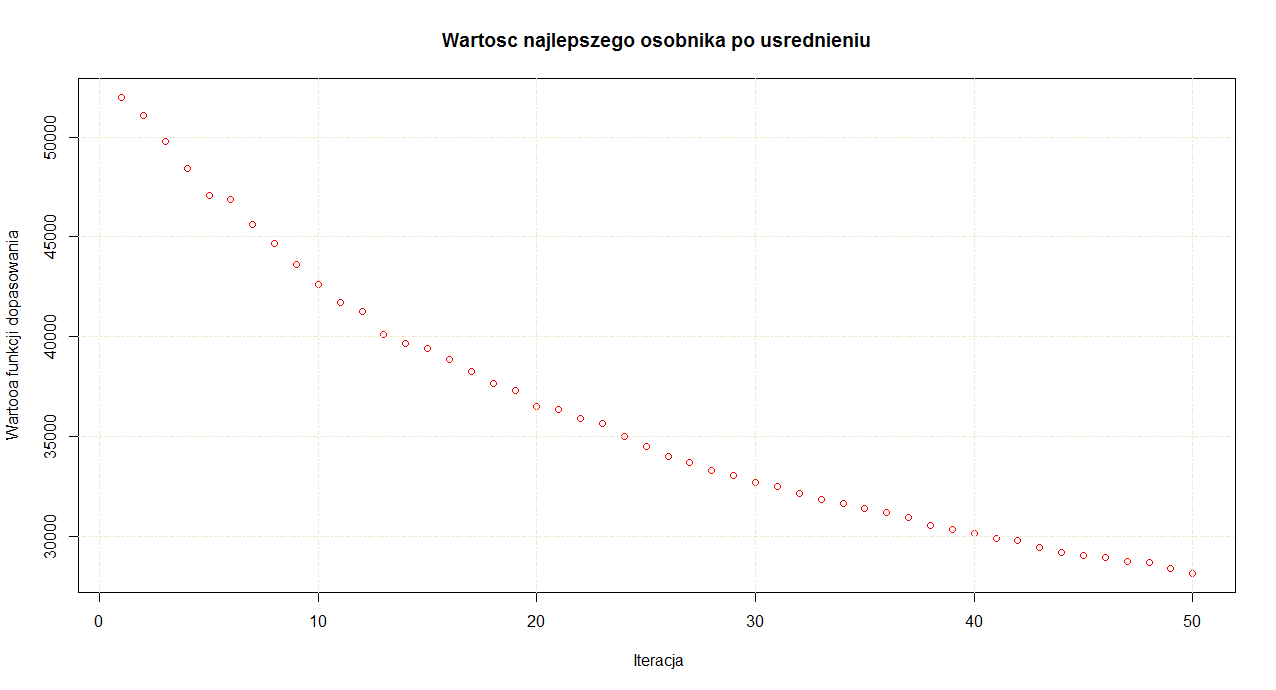
\includegraphics[scale=0.3]{IO_obrazy/US50_krz_07}
\caption{Wykres wartości najlepszego osobnika dla prawdopodobieństwa krzyżowania równego 0.7}
\end{figure}


\begin{figure}[H]
\centering

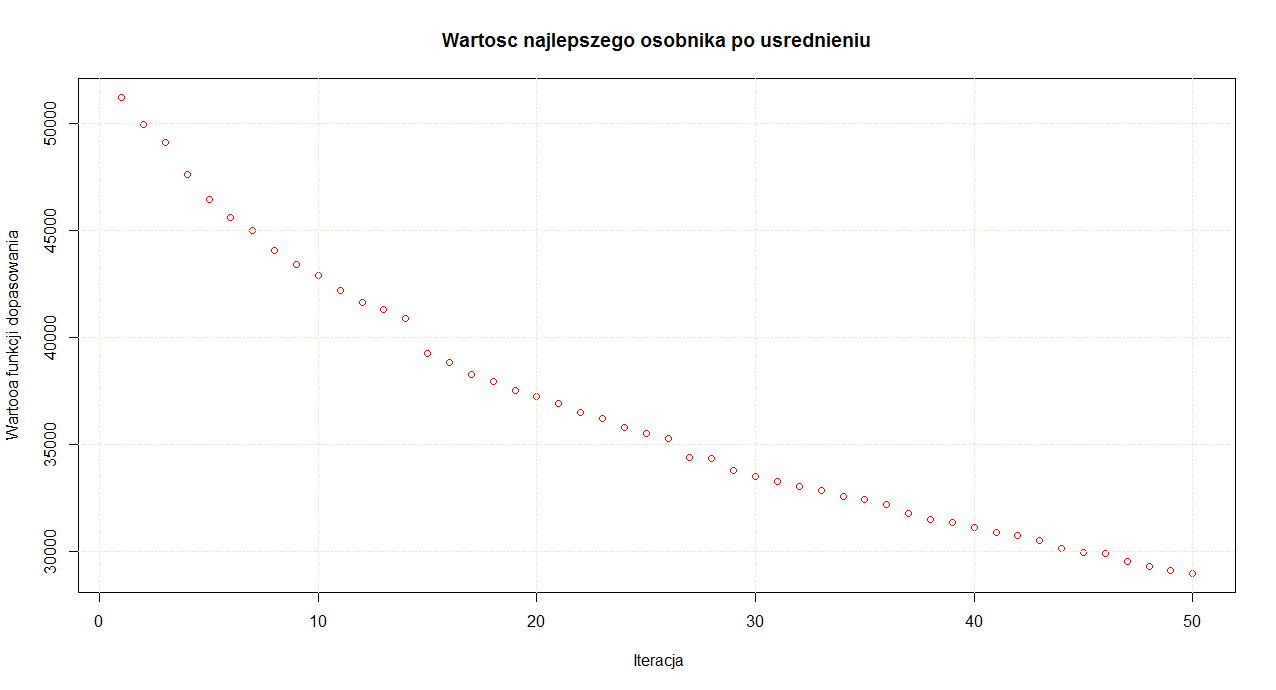
\includegraphics[scale=0.3]{IO_obrazy/US50_krz_1}
\caption{Wykres wartości najlepszego osobnika dla prawdopodobieństwa krzyżowania równego 1.0}
\end{figure}

\textbf{Podsumowanie:} Najkrótsza droga została znaleziona dla prawdopodobieństwa krzyżowania równego 0.7. 



\newpage

\subsection{Mutacja}


\begin{figure}[H]
\centering

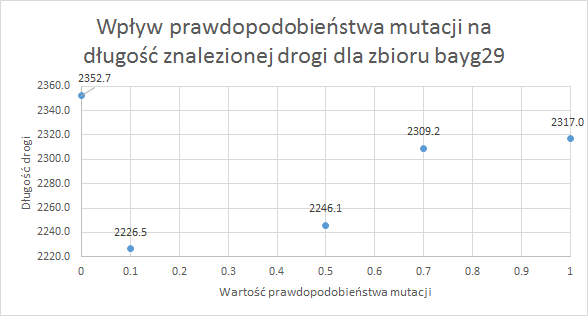
\includegraphics[scale=0.9]{IO_obrazy/excel_bayg29_mut}
\end{figure}

\begin{figure}[H]
\centering

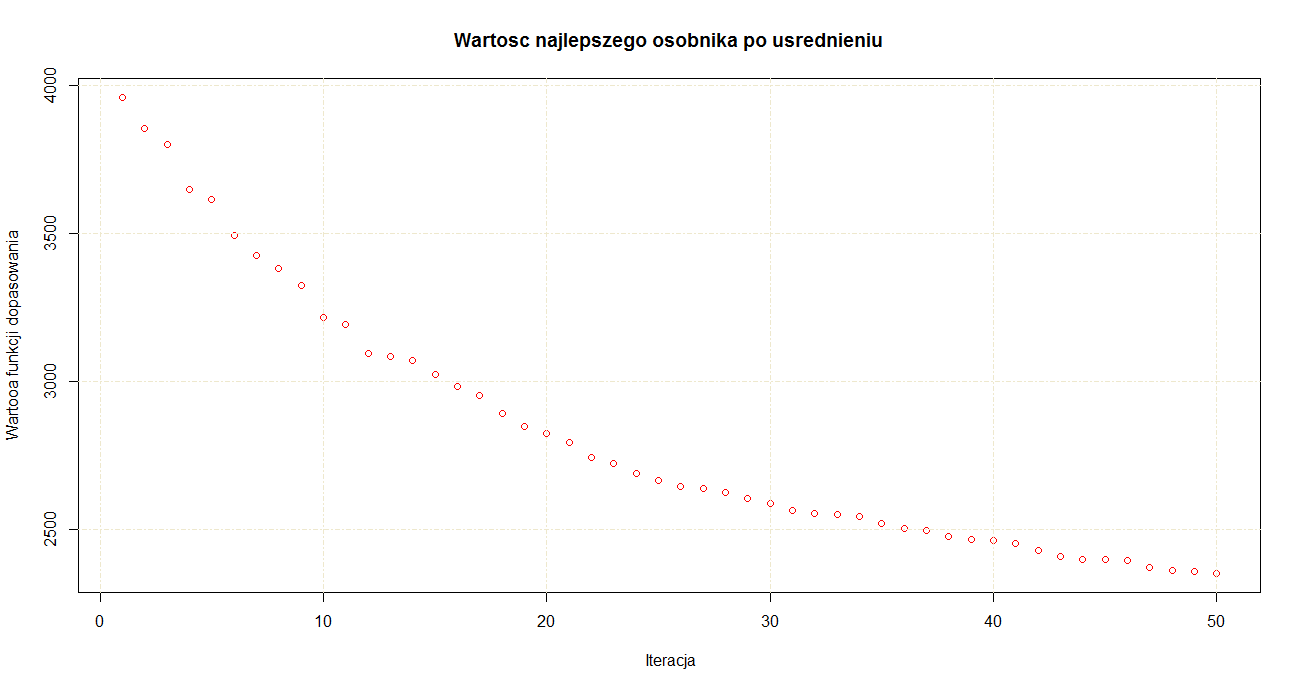
\includegraphics[scale=0.3]{IO_obrazy/bay29_mu_0}
\caption{Wykres wartości najlepszego osobnika dla prawdopodobieństwa mutacji równego 0}
\end{figure}

\begin{figure}[H]
\centering

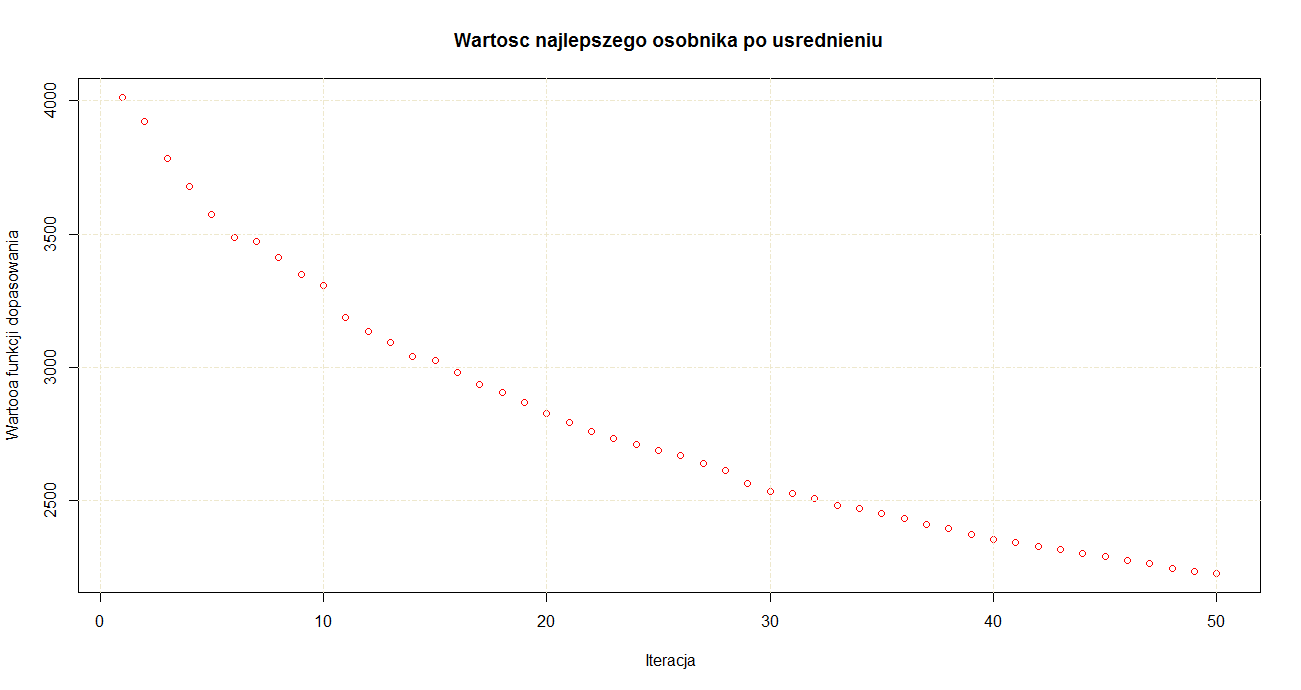
\includegraphics[scale=0.3]{IO_obrazy/bay29_mu_01}
\caption{Wykres wartości najlepszego osobnika dla prawdopodobieństwa mutacji równego 0.1}
\end{figure}

\begin{figure}[H]
\centering

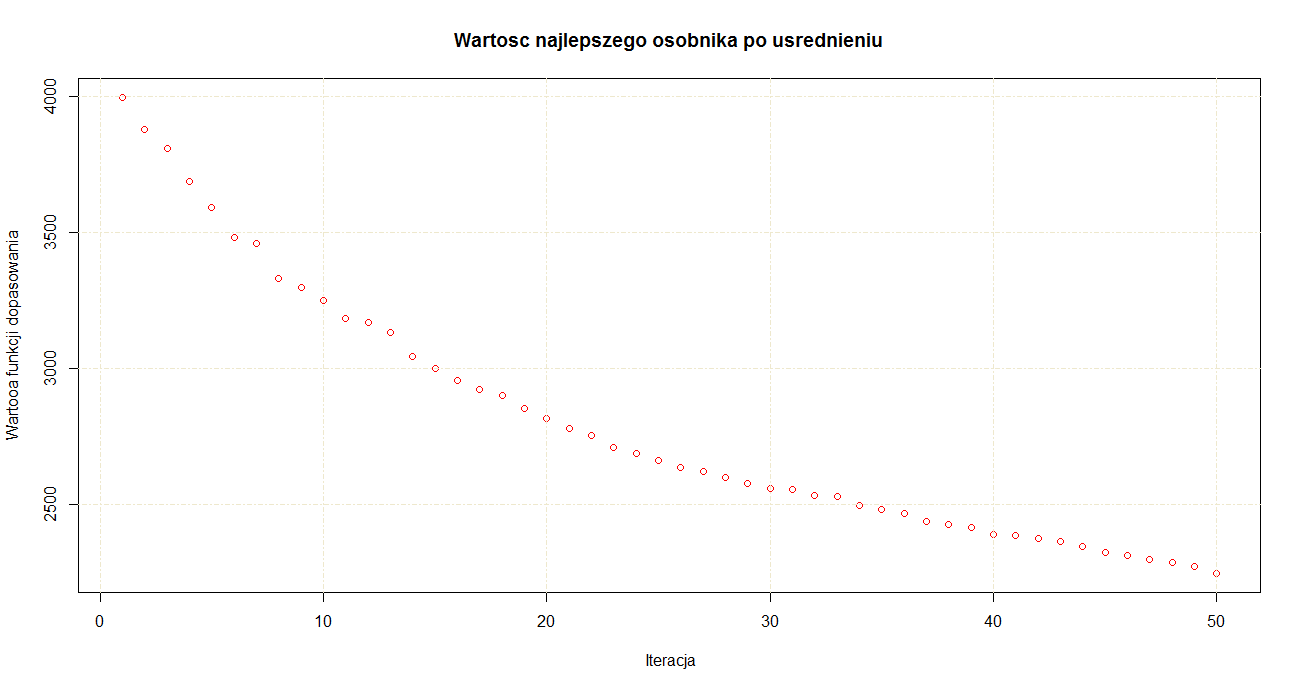
\includegraphics[scale=0.3]{IO_obrazy/bay29_mu_05}
\caption{Wykres wartości najlepszego osobnika dla prawdopodobieństwa mutacji równego 0.5}
\end{figure}

\begin{figure}[H]
\centering

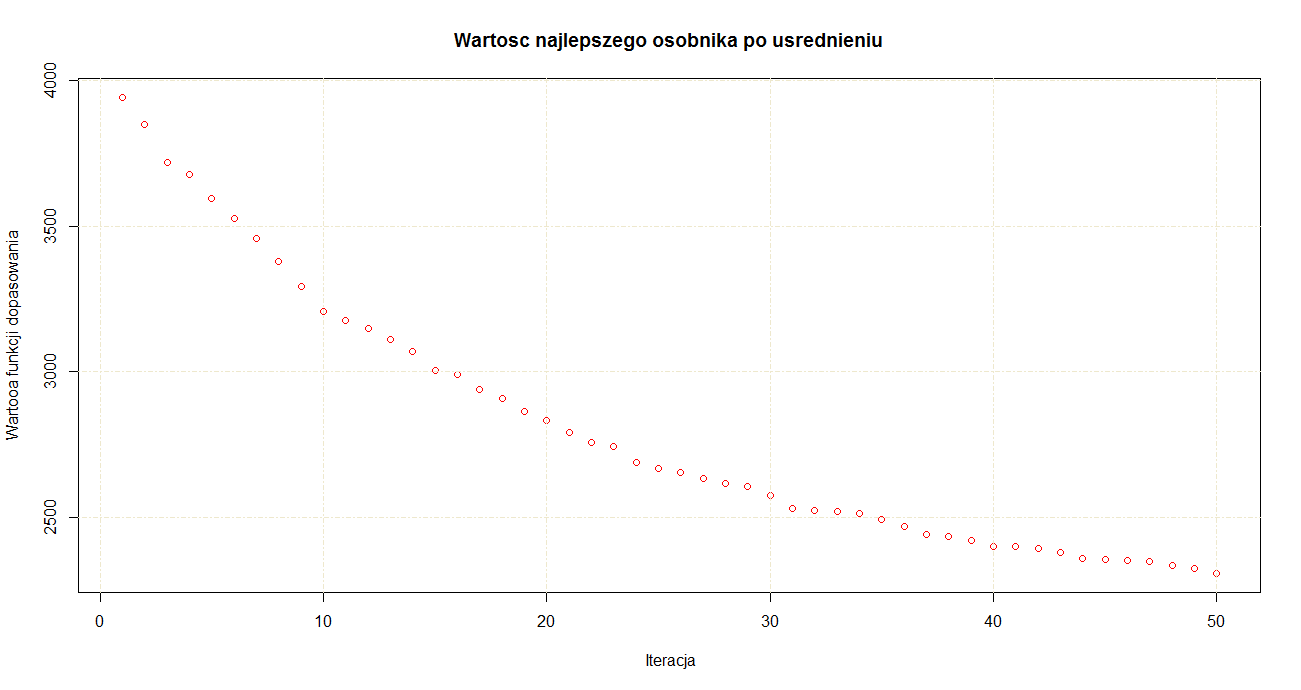
\includegraphics[scale=0.3]{IO_obrazy/bay29_mu_07}
\caption{Wykres wartości najlepszego osobnika dla prawdopodobieństwa mutacji równego 0.7}
\end{figure}


\begin{figure}[H]
\centering

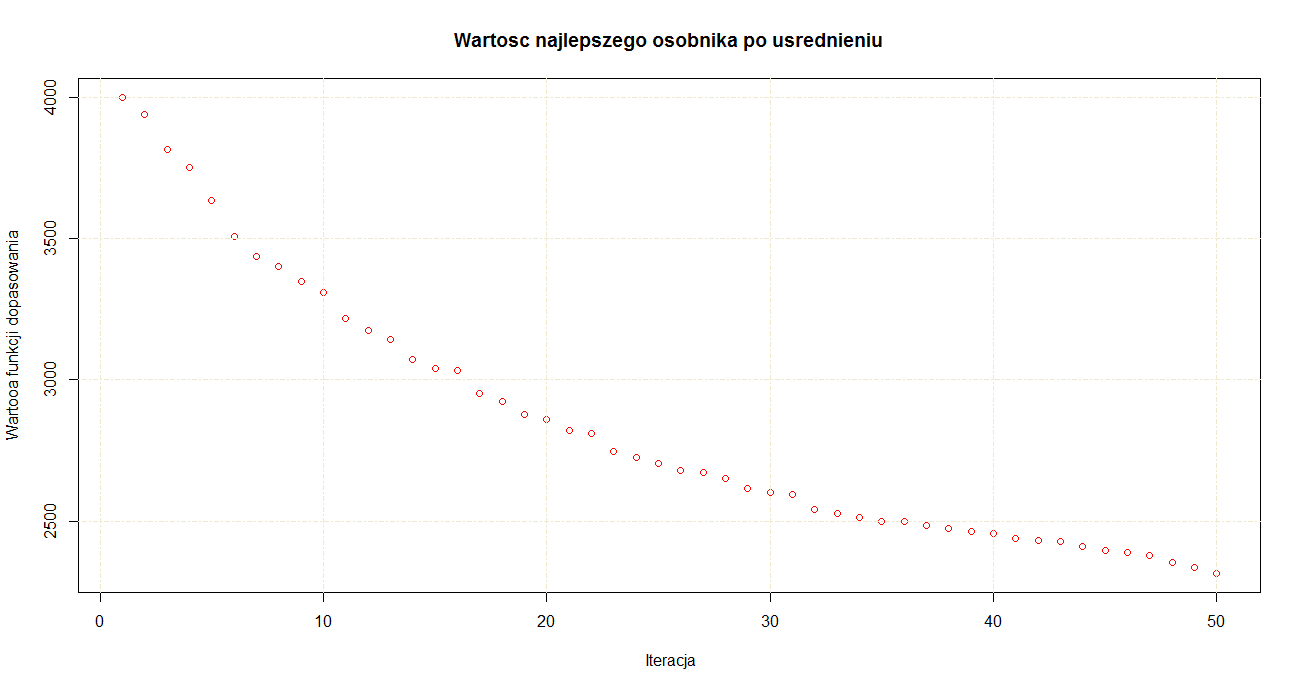
\includegraphics[scale=0.3]{IO_obrazy/bay29_mu_1}
\caption{Wykres wartości najlepszego osobnika dla prawdopodobieństwa krzyżowania równego 1}
\end{figure}

\textbf{Podsumowanie:} Najkrótsza droga została znaleziona dla prawdopodobieństwa mutacji równego 0.1 - jest to jednocześnie wartość domyślna pakietu GA.


\newpage

\subsection{Elitaryzm}

\begin{figure}[H]
\centering

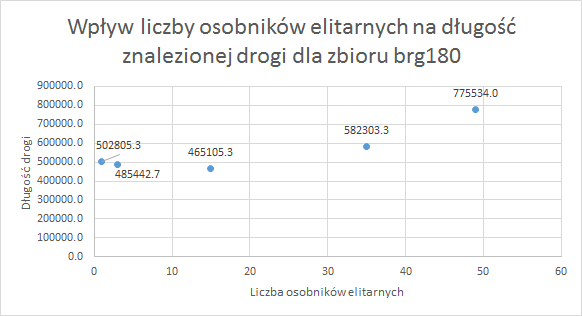
\includegraphics[scale=0.9]{IO_obrazy/excel_brg180_elit}
\end{figure}

\begin{figure}[H]
\centering

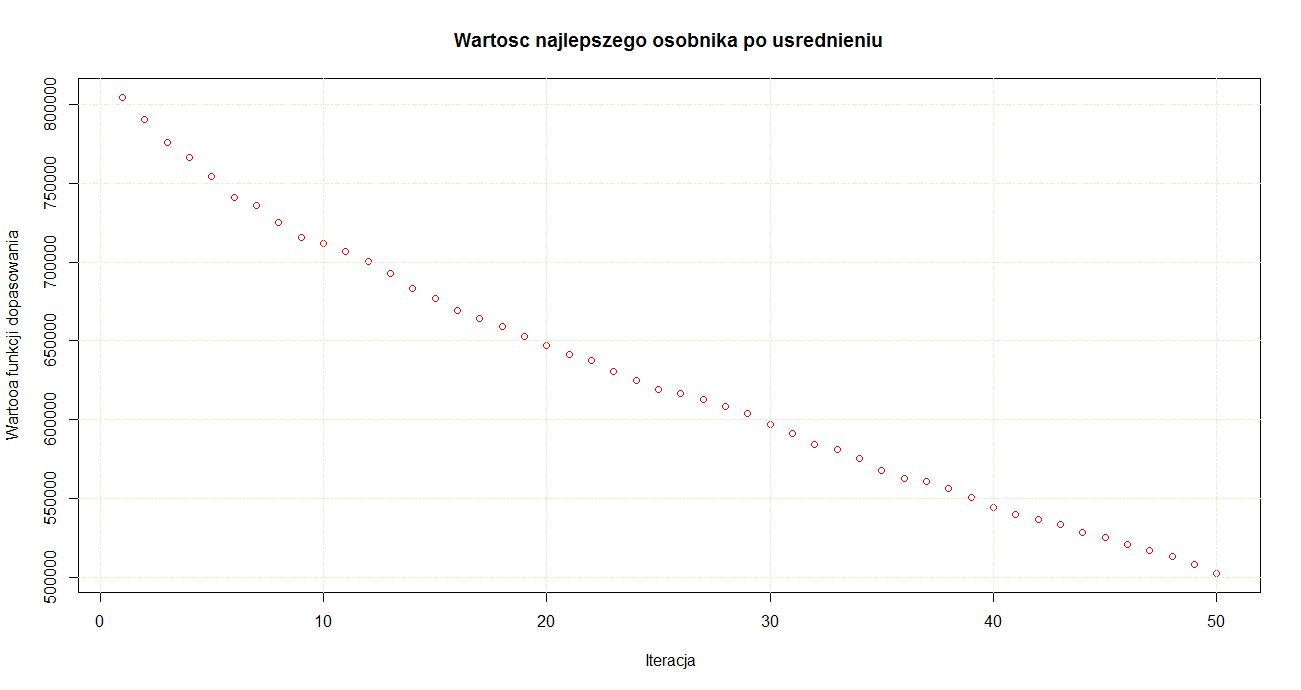
\includegraphics[scale=0.3]{IO_obrazy/brg180_elit_1}
\caption{Wykres wartości najlepszego osobnika dla liczby osobników elitarnych równej 1}
\end{figure}

\begin{figure}[H]
\centering

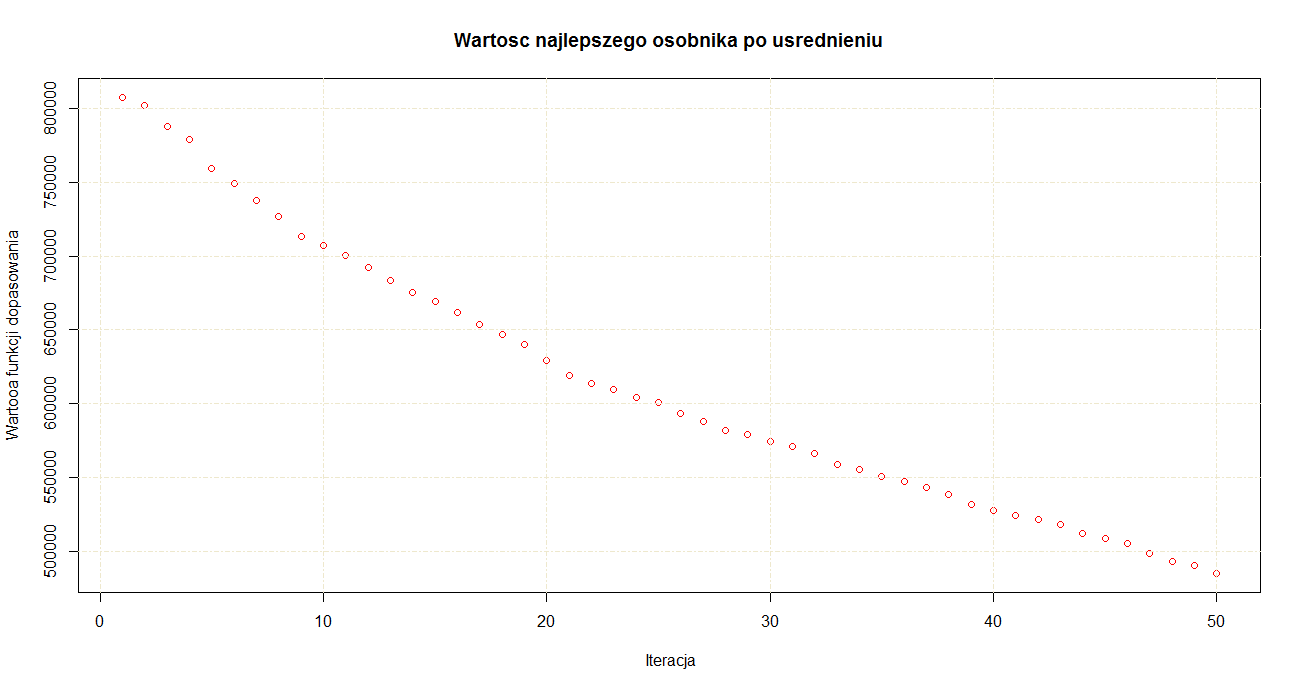
\includegraphics[scale=0.3]{IO_obrazy/brg180_elit_3}
\caption{Wykres wartości najlepszego osobnika dla liczby osobników elitarnych równej 3}
\end{figure}

\begin{figure}[H]
\centering

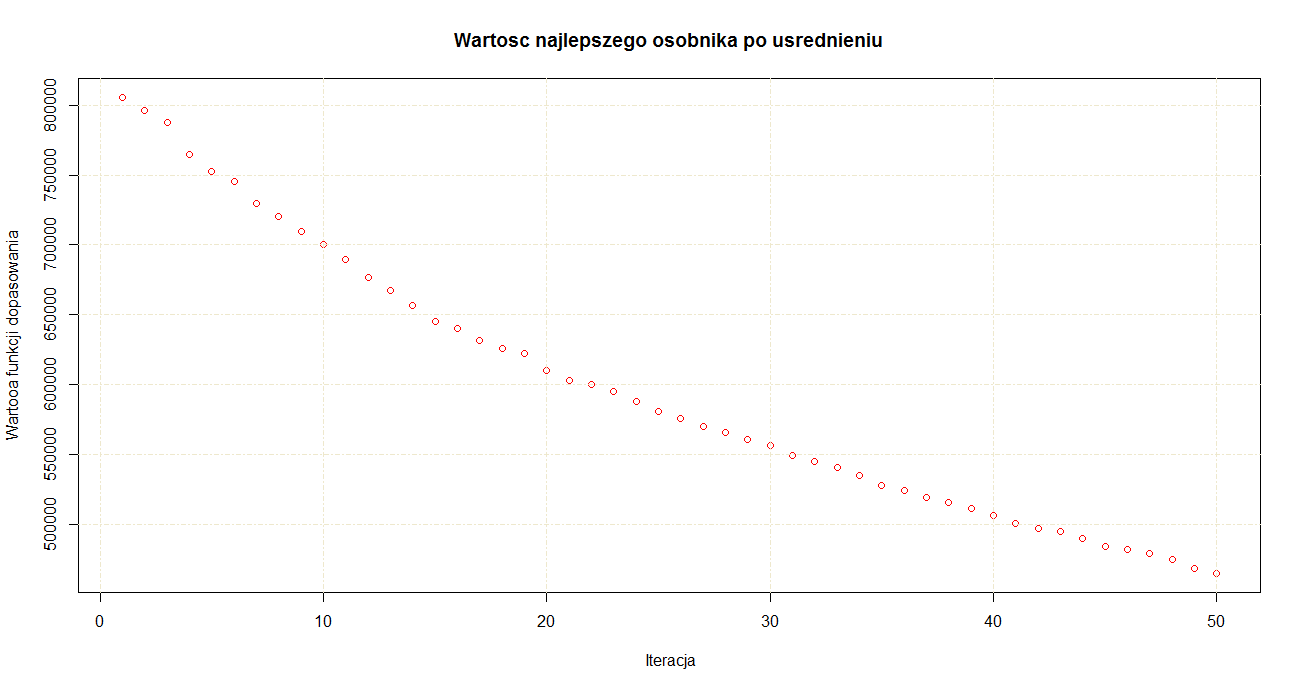
\includegraphics[scale=0.3]{IO_obrazy/brg180_elit_15}
\caption{Wykres wartości najlepszego osobnika dla liczby osobników elitarnych równej 15}
\end{figure}

\begin{figure}[H]
\centering

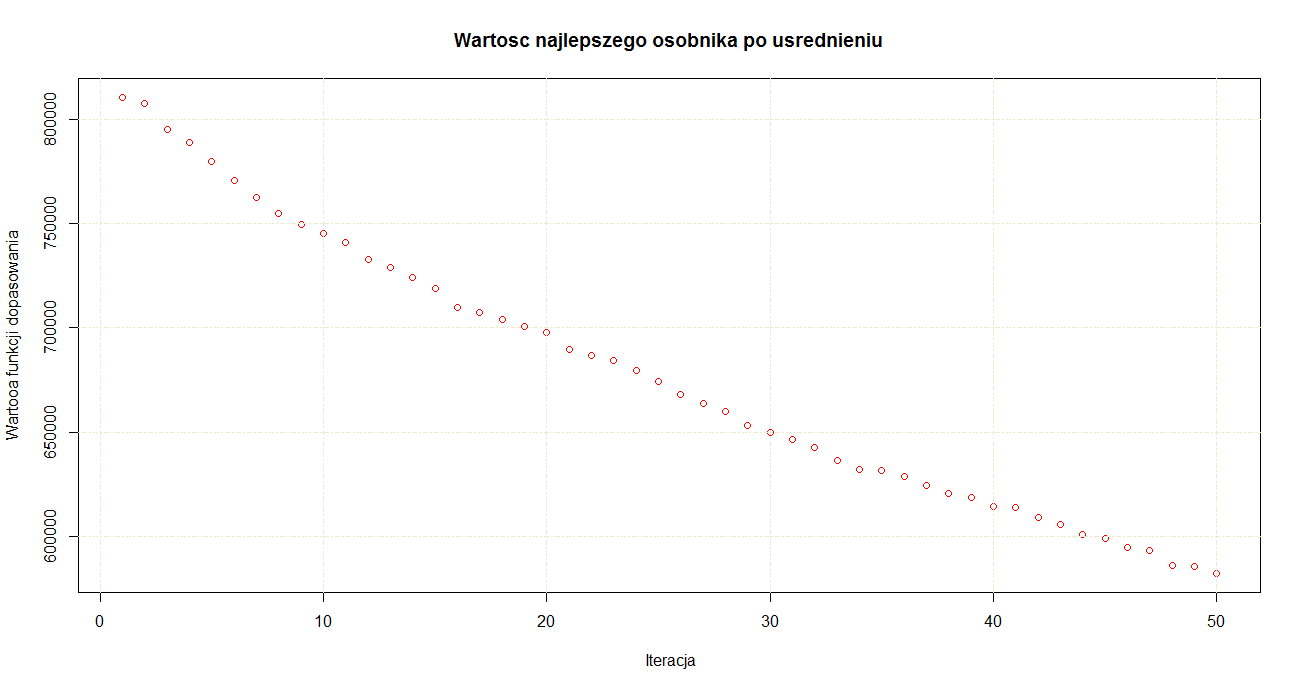
\includegraphics[scale=0.3]{IO_obrazy/brg180_elit_35}
\caption{Wykres wartości najlepszego osobnika dla liczby osobników elitarnych równej 35}
\end{figure}


\begin{figure}[H]
\centering

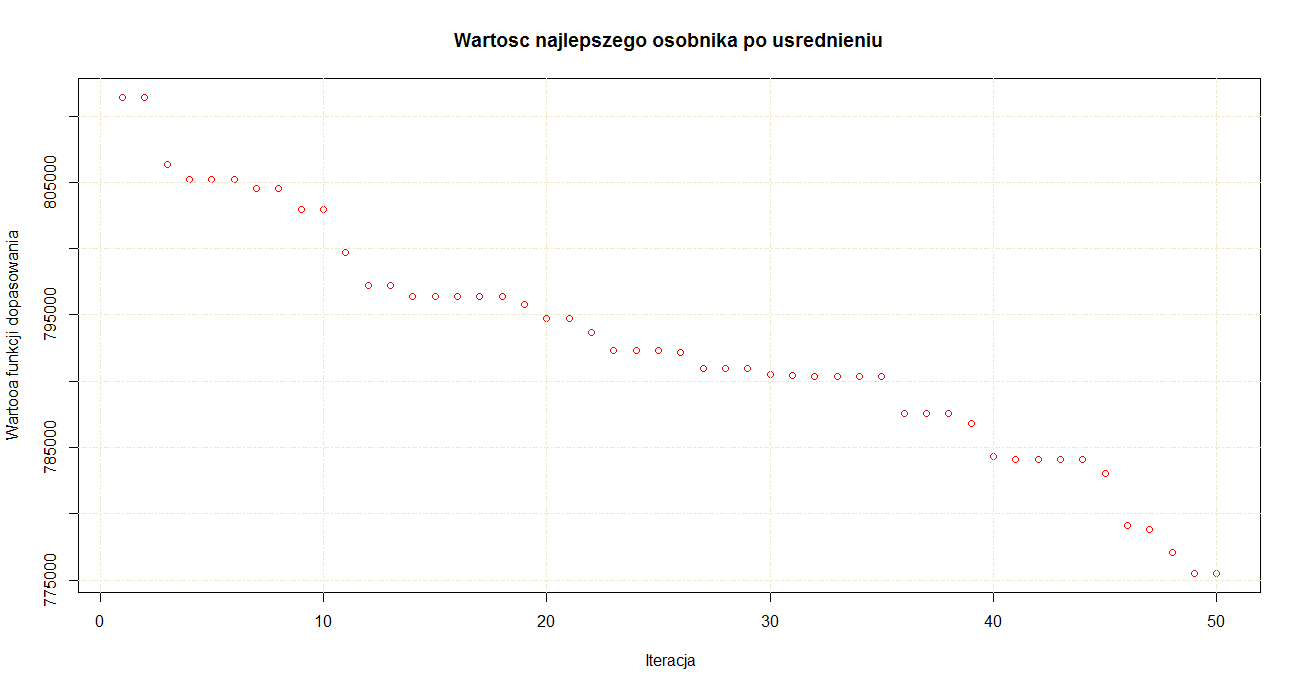
\includegraphics[scale=0.3]{IO_obrazy/brg180_elit_49}
\caption{Wykres wartości najlepszego osobnika dla liczby osobników elitarnych równej 49}
\end{figure}


\textbf{Podsumowanie}: Najkrótsza droga została znaleziona, gdy pozostawionych zostało 5 osobników elitarnych z populacji 50.

\newpage